\documentclass[10pt,twocolumn,letterpaper]{article}

\usepackage[pagenumbers]{cvpr}

\usepackage{graphicx}
\usepackage{amsmath}
\usepackage{amssymb}
\usepackage{booktabs}
\usepackage[pagebackref,breaklinks,colorlinks]{hyperref}
\usepackage[capitalize]{cleveref}
\crefname{section}{Sec.}{Secs.}
\Crefname{section}{Section}{Sections}
\Crefname{table}{Table}{Tables}
\crefname{table}{Tab.}{Tabs.}

\begin{document}

\title{Paper Review and Notes For\\DeepLab: Semantic Image Segmentation with\\Deep Convolutional Nets, Atrous Convolution, and Fully Connected CRFs}

\author{Jin Hyoung Joo\\ {\tt\small hyoungjoo.j@gmail.com} }
\maketitle

\begin{abstract}
    This paper \cite{DeepLab}
\end{abstract}

\section{Key Points}
\subsection{Proposed Methods for Segmentation}
The challenges of image segmentation and the authors' proposed method of handling
each problem can be seen as below.

\begin{itemize}
    \item{
        Atrous convolution for dense feature extraction and field-of-view enlargement
        Image segmentation needs to predict the output with reduced feature resolutions.
        The authors used \emph{atrous convolutions} (convolution with upsampled filters)
        to help with this problem.
    }
    \item{
        Image segmentation needs to segment objects at multiple scales. The authors used
        \emph{atrous spatial pyramid pooling (ASPP)} to help with this problem.
    }
    \item{
        Deep convolution networks reduce the localization accuracy due to its invariance.
        The authors used \emph{fully connected Conditional Random Fields (CRF)s} to help
        with this problem.
    }
\end{itemize}

\subsection{Advantages of DeepLab}
DeepLab has the following advantages.
\begin{itemize}
    \item{DeepLab can operate at fast speeds.}
    \item{DeepLab achieves high accuracy.}
    \item{DeepLab has a simple structure.}
\end{itemize}

\section{Technical Details}
\subsection{Atrous Convolutions}
Due to repeated combinations of pooling and downsampling, deep convolutional neural networks
significantly reduce the spatial resolution of output feature maps. Therefore, we need a method
to reduce the degree of signal downsampling. Deconvolutions can help with this problem with
the cost of additional memory and time.

\emph{Atrous convolutions (Dilated convolutions)} allow computing the responses of any
layer at any desirable resolution. This operation is done by convolving through a
sequence, where the values are sampled with a stride of $r$.
\[
    y[i] = \sum_{k=1}^K{x[i + rk]w[k]}
\]

Atrous convolutions increase the effecive field-of-view of filters.

using atrous convolution to increase by a factor of 4 the den- sity of computed feature maps, followed by fast bilinear interpolation by an additional factor of 8 to recover feature maps at the original image resolution

\begin{figure}[ht]
  \centering
   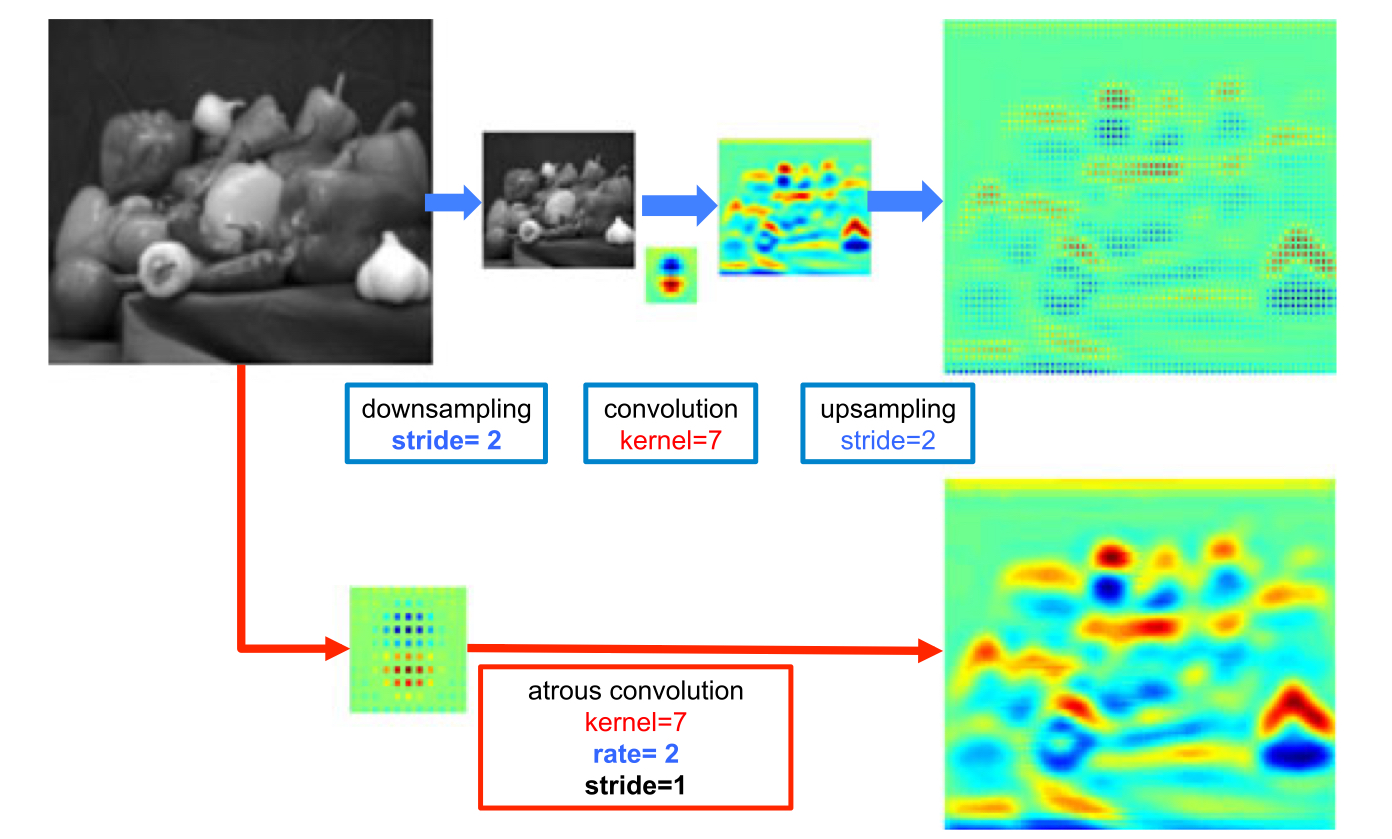
\includegraphics[width=\linewidth]{figures/atrous-convolution.jpeg}
   \caption{Benefit of atrous convolutions. By using the same filter size, atrous convolutions
       compute responses at all image positions. This leads to a higher quality output feature
       map without increasing the number of parameters or operations.
   }
\end{figure}

implicitly upsample the filters by inserting holesimplicitly upsample the filters by inserting holes
sparsely sample the input feature maps

This is done by either upsampling the kernel filter or by upsampling the input image by
inserting zeros.

\subsection{Atrous Spatial Pyramid Pooling}
Explicitly accounting for object scale can improve a model's ability to handle both
small and large objects. The authors used standard multiscale processing and the
proposed atrous spatial pyramid pooling (ASPP) method.

The standard multiscale processing runs multiple rescaled version of the input on 
the entire model, and then fusing the output feature maps. This improves performance,
but at the cost of executing the model multiple times for a single input.

Atrous spatial pyramid pooling uses multiple parallel atrous convolution layers
with different sampling rates. Each of these features are fused together to output
a feature map.

\begin{figure}[ht]
  \centering
   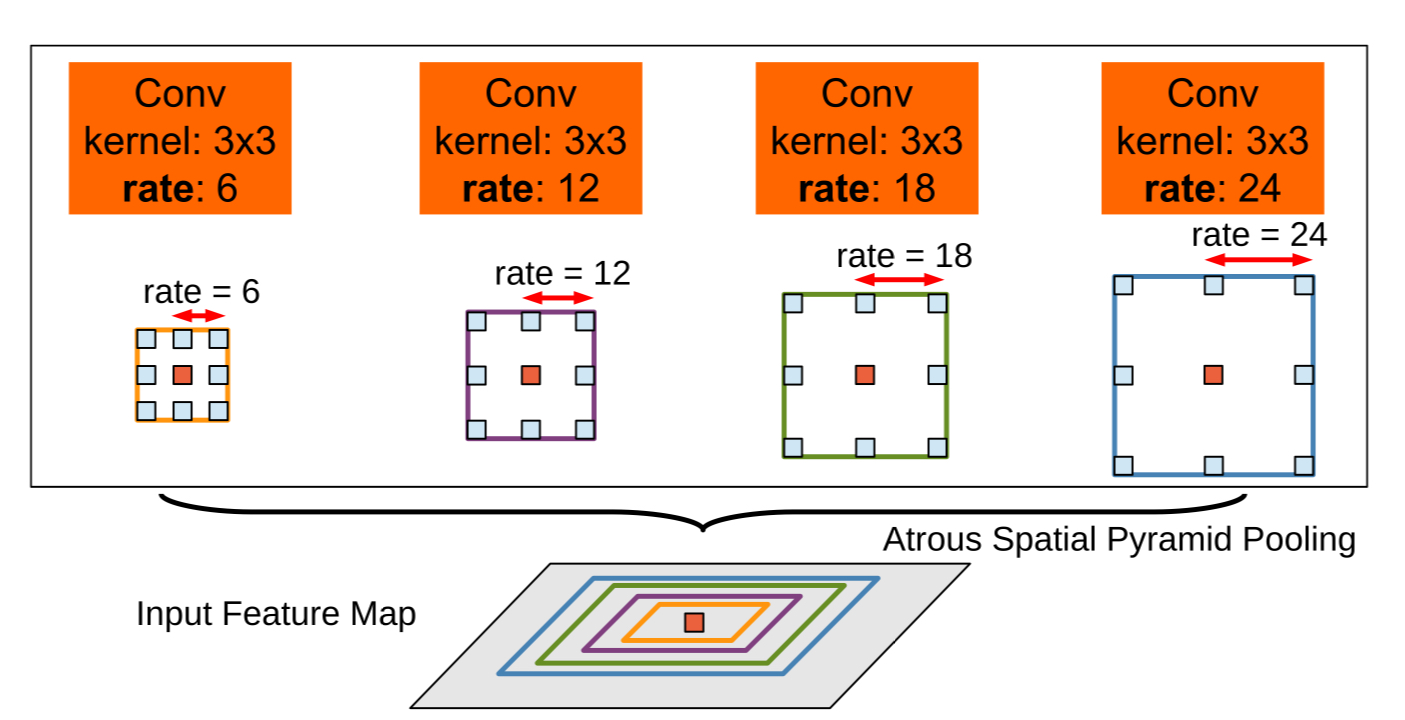
\includegraphics[width=\linewidth]{figures/ASPP.jpeg}
   \caption{Atrous spatial pyramid pooling. A single pixel is computed by multiple
       feature maps with different reception fields.
   }
\end{figure}

\subsection{Fully Connected CRFs}
For deep convolutional neural networks, a trade-off between localization accuracy and
classification performance exists. The authors aimed to use the recognition capability
of convolutional networks and the fine-grained localization accuracy of fully-connected
CRFs.
\[
    E(x) = \sum_i {\theta_i (x_i)} + \sum_{ij} \theta_{ij}{(x_i, x_j)}
\]
\[
    \theta_i (x_i) = -\log P(x_i)
\]
\[
    \theta_{ij}(x_i, x-j) = \mu(x_i, x_j)\left[
        w_1 exp(-\frac{\|p_i - p_j\|^2}{2\sigma^2_\alpha} -\frac{\|I_i - I_j\|^2}{2\sigma^2_\beta})
        + w_2 exp(-\frac{\|p_i - p_j\|^2}{2\sigma^2_\gamma})
    \right]
\]

\section{Further Research}

{\small \bibliographystyle{cite-style} \bibliography{citations} }

\end{document}


